% ---------------------------------------------------
%
% Trabajo de Fin de Grado. 
% Author: Adriano dos Santos Moreira <alu0101436784@ull.edu.es>
% Chapter: Benchmark Comparisons
% File: Cap4_Benchmark_Comparisons.tex
%
% ----------------------------------------------------
%

\chapter{Benchmark Comparisons} \label{chap:Benchmark_Comparisons} 

In this chapter, we will run and compare various benchmarks using SYCL, CUDA and sequential CPU executions.
For this purpose, we will use \textit{HeCBench}\footnote{\href{https://github.com/zjin-lcf/HeCBench/}{{HeCBench} \url{https://github.com/zjin-lcf/HeCBench/}}}, an assortment of benchmarks specialised in heterogeneous computation.
HecBench offers over 400 different benchmarks written in HIP, OpenMP, CUDA and SYCL.

The objective of this study is to examine the practical differences between SYCL, CUDA, and serial executions in terms of performance.
Consequently, we will only provide a brief description of the algorithms and concepts used in this chapter.
For the benchmarks presented we will not go into the details of the SYCL parallelisation of the code. 
For details of the code in both CUDA and SYCL, the interested reader is referred to the source code available in the HeCBench repository for these algorithms.
In Chapter \ref{chap:CaseStudy}  we will present computational results accompanied by a comparison of SYCL and CUDA implementations for other algorithms.

Since this work serves as an introduction to heterogeneous computation and we aim to present a simplified benchmark report, we will only experiment with problem sizes in order to execute the benchmarks, with the rest of the parameters remaining at their default values.

Lastly, the graphs created for these benchmarks were plotted using Python and MatplotLib\footnote{\href{https://matplotlib.org}{{MatplotLib} \url{https://matplotlib.org}}} among other Python utilities.

\section{Execution Platform}
The experiments shown in this chapter have been executed on the \textit{Verode} platform, a computing infrastructure belonging to the High Performance Computing Group (\textit{Grupo de Computación de Altas Prestaciones} or \textit{GCAP})\footnote{\href{https://portalciencia.ull.es/grupos/6369/detalle}{{ULL GCAP} \url{https://portalciencia.ull.es/grupos/6369/detalle}}} of the Universidad de La Laguna.

\textit{Verode} is equipped with two Intel® Xeon® CPU Gold 6230N processors,  with 20 cores each, for a total of 40 cores using shared memory, this platform also provides an NVIDIA Tesla V100 GPU, especially designed for HPC and data science purposes.

Regarding the software specifications:
\begin{itemize}
    \item \textit{Verode} runs under the Debian GNU/Linux 11 (bullseye) operating system.
    \item SYCL programs were compiled using:
    \begin{itemize}
        \item \texttt{clang++} version 18.0.0.
        \item \texttt{gcc} version 12.3.0 for the GCC toolchain.
    \end{itemize}
    \item CUDA programs were compiled using:
        \begin{itemize}
            \item \texttt{nvcc} version 12.0.
            \item \texttt{gcc} version 6.5.0 as the host compiler.
        \end{itemize}
\end{itemize}

\section{Mandelbrot set}
The Mandelbrot set is a mathematical concept that was first described by Benoit Mandelbrot in 1980.
It is an infinite and infinitely complex fractal shape that emerges from a simple equation involving complex numbers.

For this specific benchmark, we had to make a small change in the code to be able to modify the size of the Mandelbrot set region.
As a result, this benchmark offers two parameters to experiment with:
\begin{itemize}
    \item \texttt{repeat}: How many times the algorithm is repeated, then averaged over all times. Using a fixed amount of 1000.
    \item \texttt{size}: Side length of the Mandelbrot set region. It always calculates a square area. Using sizes from 1000 to 45000.
\end{itemize}

Figure \ref{fig:mandelbrot-benchmark-all} shows the results for SYCL, CUDA and serial executions.

\begin{figure}[H]
	\centering
	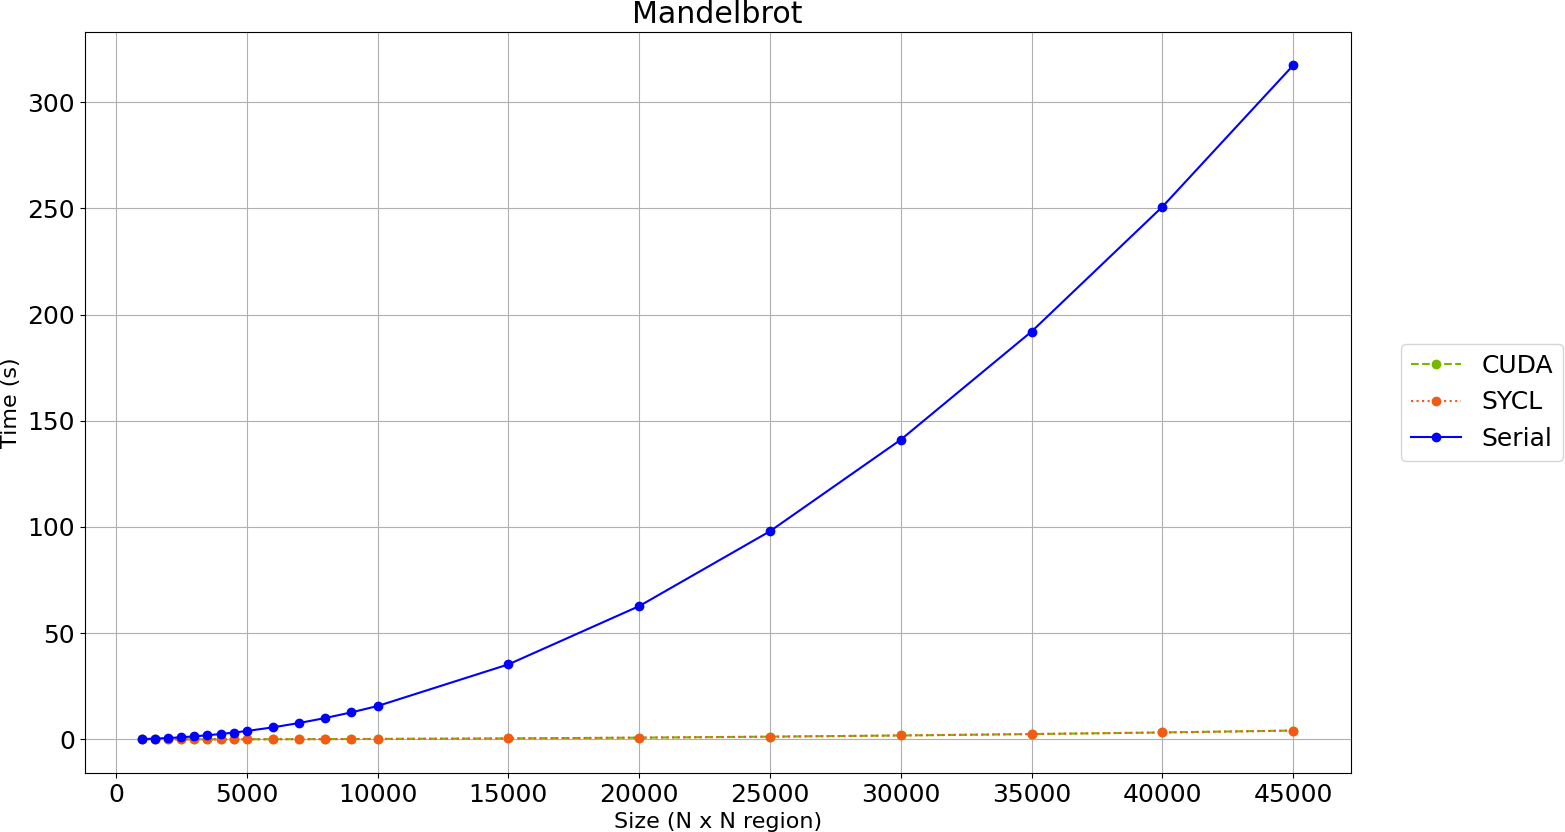
\includegraphics[width=\linewidth]{images/mandelbrot-sycl-cuda-serial.png}
	\caption{Mandelbrot benchmark. Results for SYCL, CUDA and serial executions.}
	\label{fig:mandelbrot-benchmark-all}
\end{figure}

Naturally, we can see in Figure \ref{fig:mandelbrot-benchmark-all} that CUDA and SYCL times are significantly better than serial times, reaching a gigantic time gap of over 300 seconds at size 45000.

On the other hand, in Figure \ref{fig:mandelbrot-benchmark-parallel} we can barely notice any differences when comparing the execution times of SYCL and CUDA, which speaks in favour of SYCL since it offers a higher abstraction and justifies any potential performance loss.

\begin{figure}[H]
	\centering
	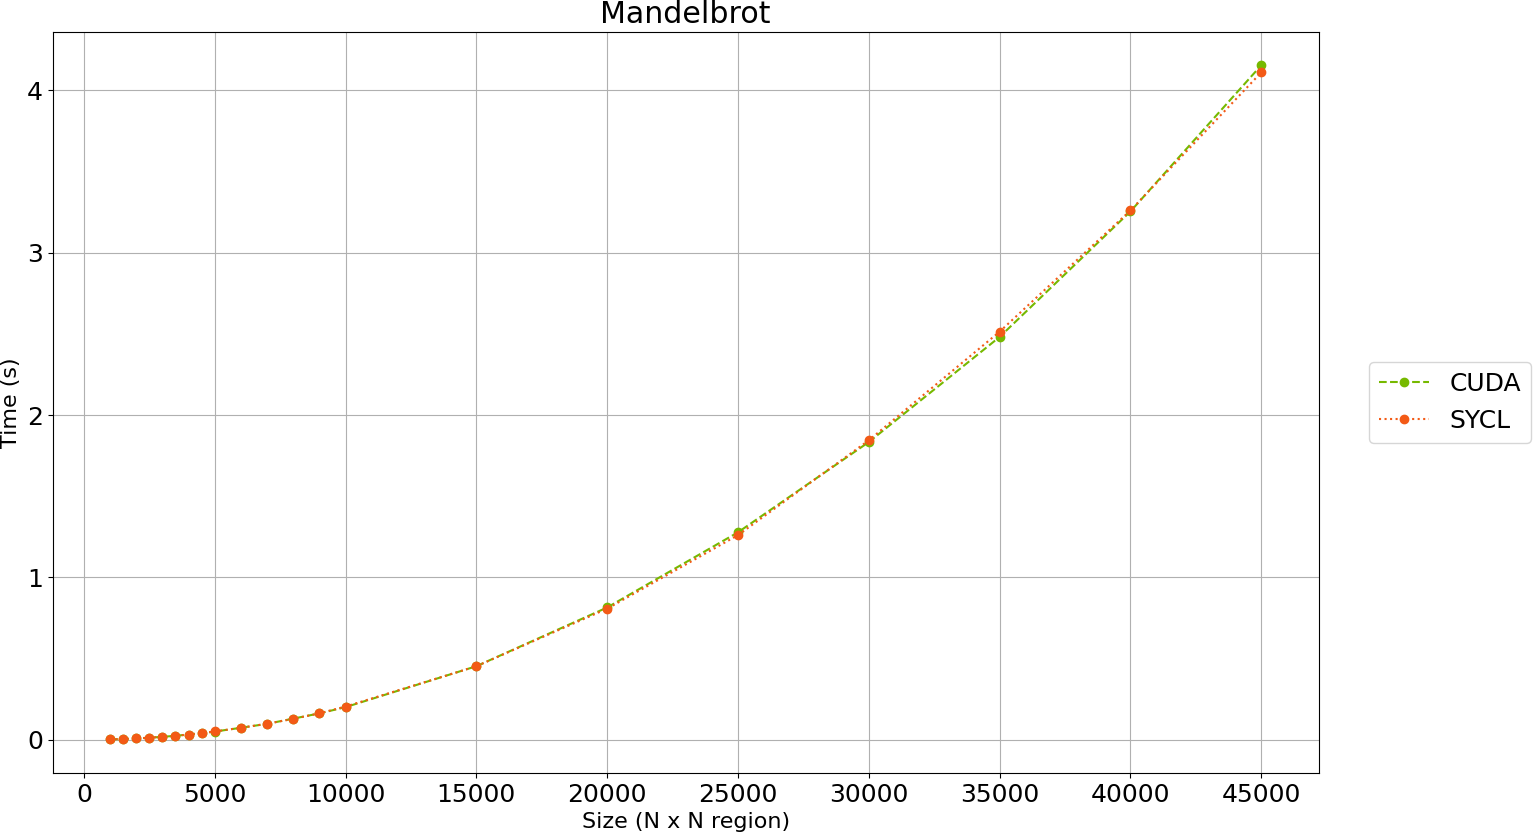
\includegraphics[width=\linewidth]{images/mandelbrot-sycl-cuda.png}
	\caption{Mandelbrot benchmark. Results for SYCL and CUDA executions.}
	\label{fig:mandelbrot-benchmark-parallel}
\end{figure}

In Figure \ref{fig:mandelbrot-speed-up}, it is observed that the speed up achieved decreases slightly as the size of the problem increases.
Again, we can see that both SYCL and CUDA results are fairly similar, although they seem to fluctuate a little.

\begin{figure}[H]
	\centering
	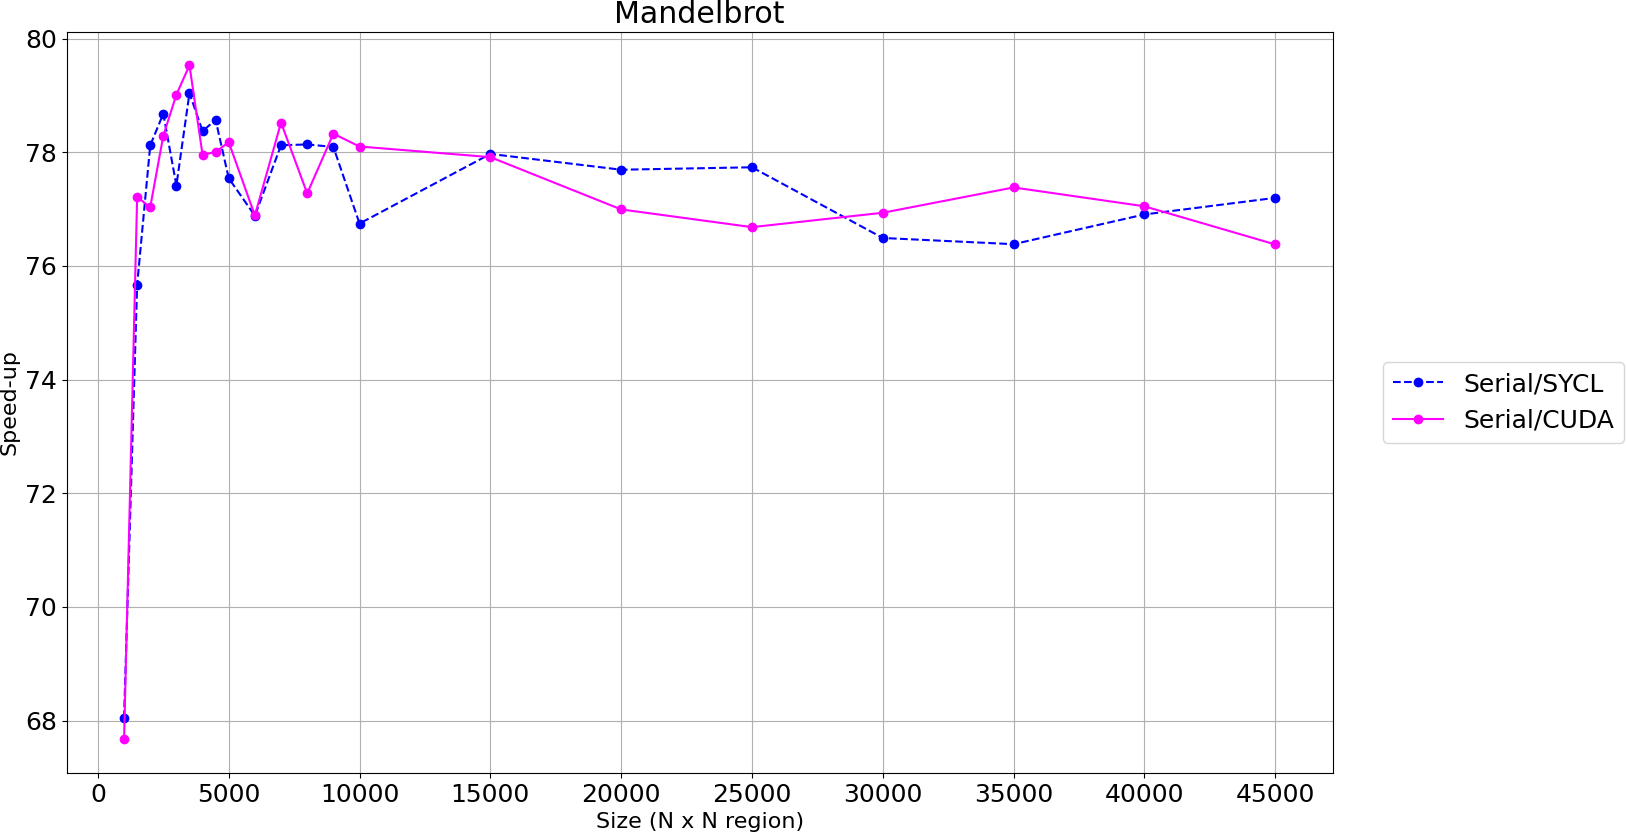
\includegraphics[width=\linewidth]{images/mandelbrot-speed-up-sycl-cuda.png}
	\caption{Mandelbrot benchmark. Speed-up graph for SYCL and CUDA executions.}
	\label{fig:mandelbrot-speed-up}
\end{figure}

\section{Floyd–Warshall algorithm}

The Floyd-Warshall algorithm is a method used to find the shortest paths in a weighted graph, where the weight of each edge represents the distance between two vertices.
Unlike other shortest path algorithms like Dijkstra's algorithm, Floyd-Warshall works for graphs with negative edge weights, as long as there are no negative cycles.

These are the parameters we can work with:
\begin{itemize}
    \item \texttt{iterations}: How many times the algorithm is repeated, then averaged over all times. Using a fixed amount of 100.
    \item \texttt{block size}: Block size used in the NDRange. Using a fixed amount of 16.
    \item \texttt{number of nodes}: Amount of nodes in the weighted graph. Using 500 to 10000 nodes.
\end{itemize}

Figure \ref{fig:floydwarshall-benchmark-all} presents the resulting graph for SYCL, CUDA and serial executions.

\begin{figure}[H]
	\centering
	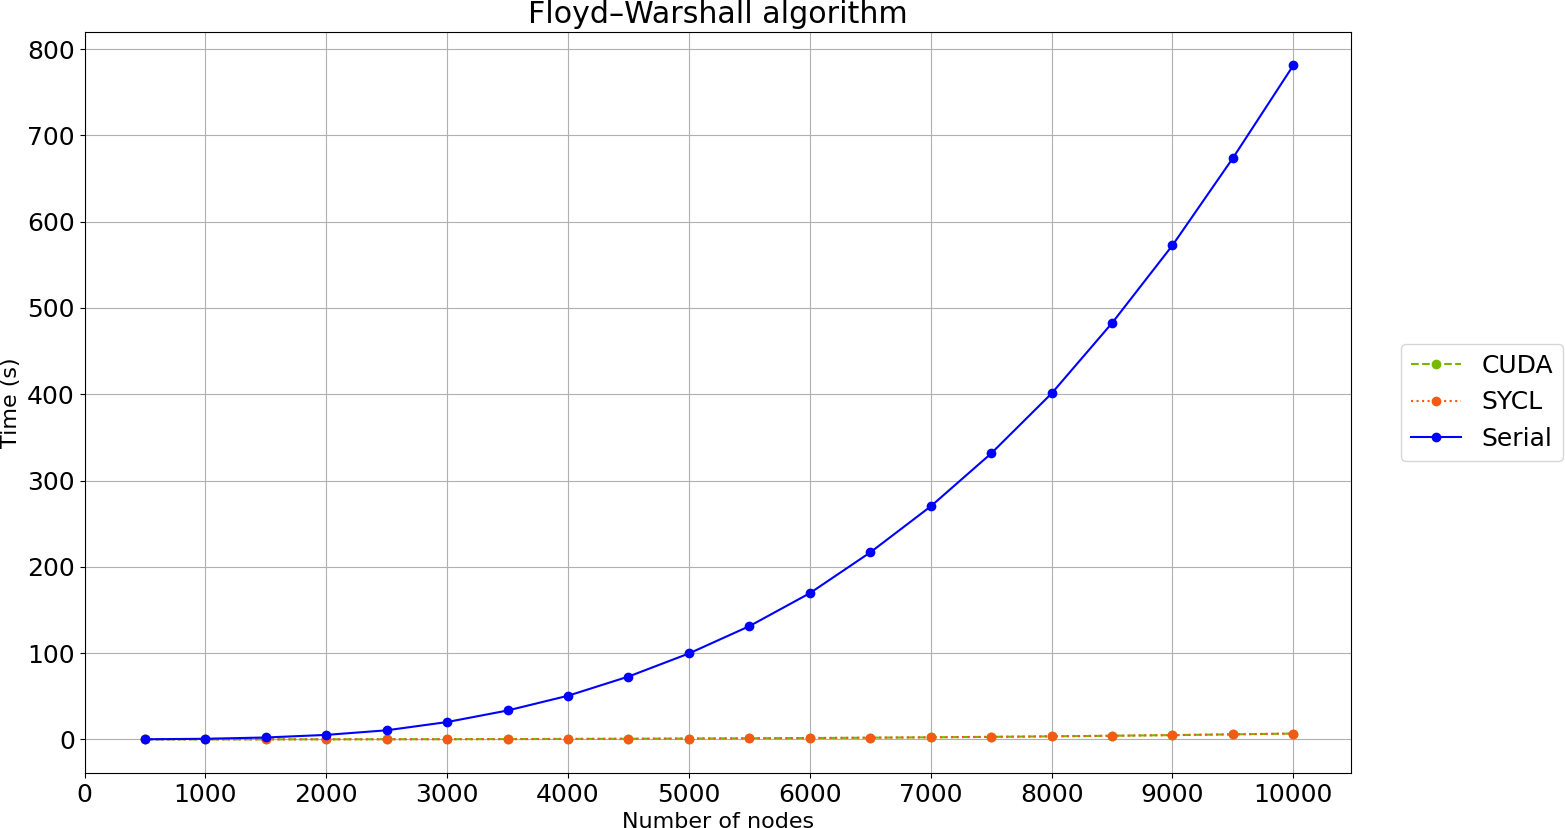
\includegraphics[width=\linewidth]{images/floydwarshall-sycl-cuda-serial.png}
	\caption{Floyd–Warshall algorithm. Results for SYCL, CUDA and serial executions.}
	\label{fig:floydwarshall-benchmark-all}
\end{figure}

The resulting graph in Figure \ref{fig:floydwarshall-benchmark-all} clearly demonstrates that serial execution is significantly slower than both SYCL and CUDA implementations as the problem size increases.

A closer examination of SYCL and CUDA graphs (Figure \ref{fig:floydwarshall-benchmark-parallel}) reveals that most execution instances exhibit a high degree of similarity in terms of execution time.
However, the last three problem sizes show the greatest differences, although these are not too significant.

\begin{figure}[H]
	\centering
	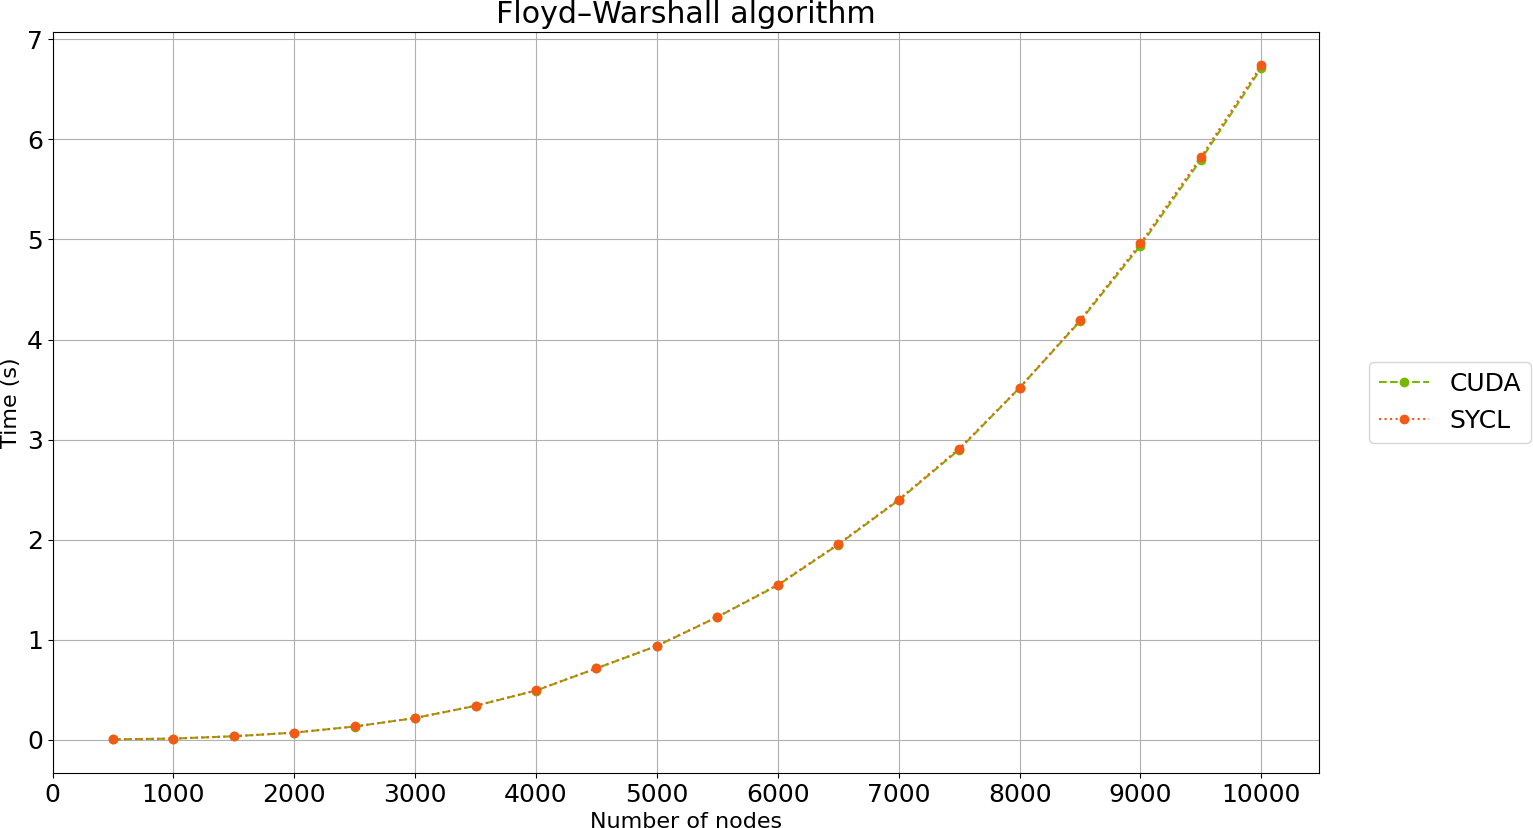
\includegraphics[width=\linewidth]{images/floydwarshall-sycl-cuda.png}
	\caption{Floyd–Warshall algorithm benchmark graph for SYCL and CUDA executions.}
	\label{fig:floydwarshall-benchmark-parallel}
\end{figure}

In terms of speed-up, Figure \ref{fig:floydwarshall-speed-up} reflects an almost identical graph for SYCL and CUDA, tracing a logarithmic-like representation in both cases.

\begin{figure}[H]
	\centering
	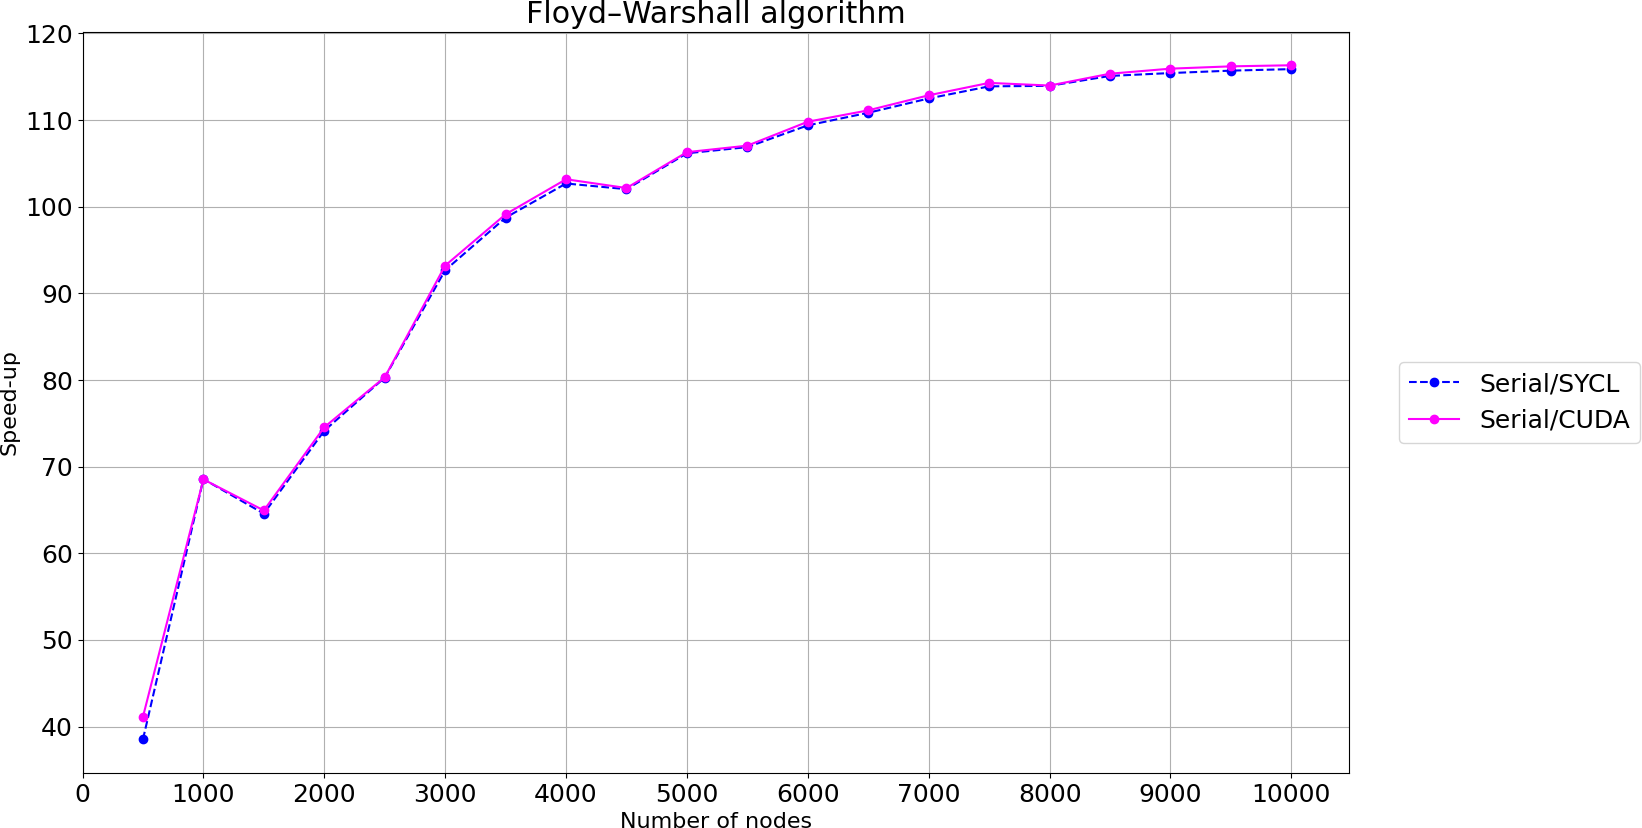
\includegraphics[width=\linewidth]{images/floydwarshall-speed-up-sycl-cuda.png}
	\caption{Floyd–Warshall algorithm speed-up graph for SYCL and CUDA executions.}
	\label{fig:floydwarshall-speed-up}
\end{figure}

\section{Molecular dynamics}
Molecular dynamics (MD) is a powerful computational simulation technique used to study the physical movements of atoms and molecules over time.
By applying the principles of classical mechanics, MD allows scientists to predict the behavior of matter at the molecular level, offering insights into the structural, dynamic, and thermodynamic properties of complex systems such as proteins, nucleic acids, and materials.

Once more, the original benchmark had to be slightly modified to be able to input different problem sizes.
There are two parameters we can work with:
\begin{itemize}
    \item \texttt{problem size}: Number of atoms in the simulation. Using sizes 2500 to 1000000.
    \item \texttt{iterations}: How many times the MD kernel is executed, then averaged over all times. Using a fixed amount of 1000.
\end{itemize}

\begin{figure}[H]
	\centering
	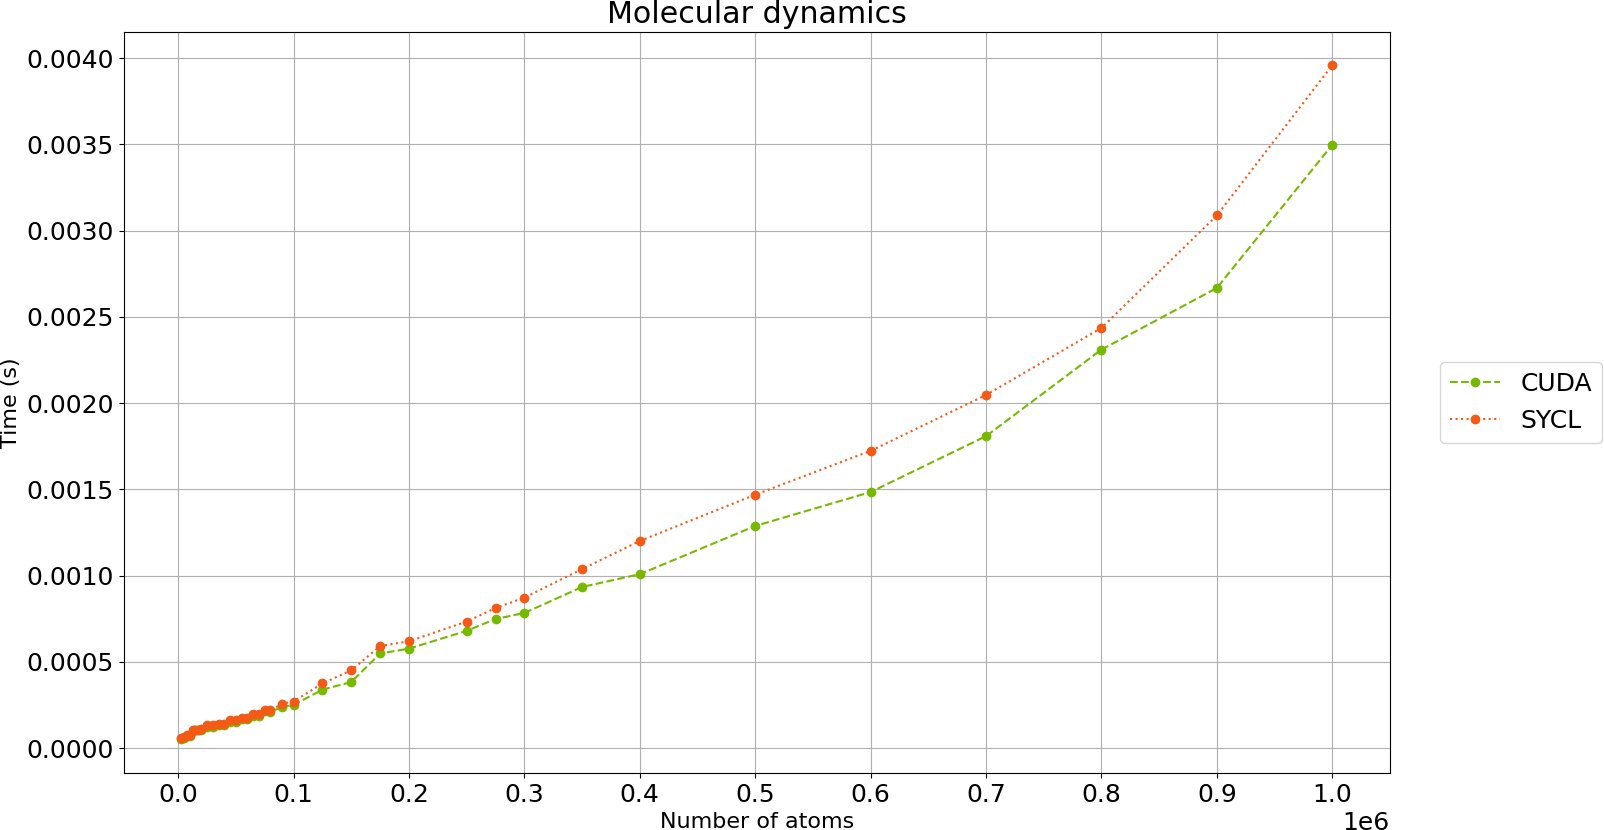
\includegraphics[width=\linewidth]{images/md-sycl-cuda.png}
	\caption{MD benchmark. Results for SYCL and CUDA executions.}
	\label{fig:md-sycl-cuda}
\end{figure}

In Figure \ref{fig:md-sycl-cuda} we measured the average kernel execution time for each selected size.
From this graph we can see that both implementations run at similar speeds, although CUDA becomes up to 11.65\% faster (on problem size 1000000) than SYCL as the number of atoms increases.

\section{Backpropagation}
Backpropagation, is a fundamental algorithm in machine learning, particularly in the training of artificial neural networks.
It enables the development of complex models that can perform tasks such as image recognition and natural language processing.
The algorithm works by iteratively adjusting the weights of the network to minimize the difference between the predicted output and the actual target output, which is measured by a loss function.

In this case, the algorithm has a single parameter: the \texttt{number of input nodes} (number of nodes in the neural network). The code requires a value divisible by 16 and for these experiments the value ranges from 512 to 1024000. 
What is being measured is the device offloading time for all execution instances.

\begin{figure}[H]
	\centering
	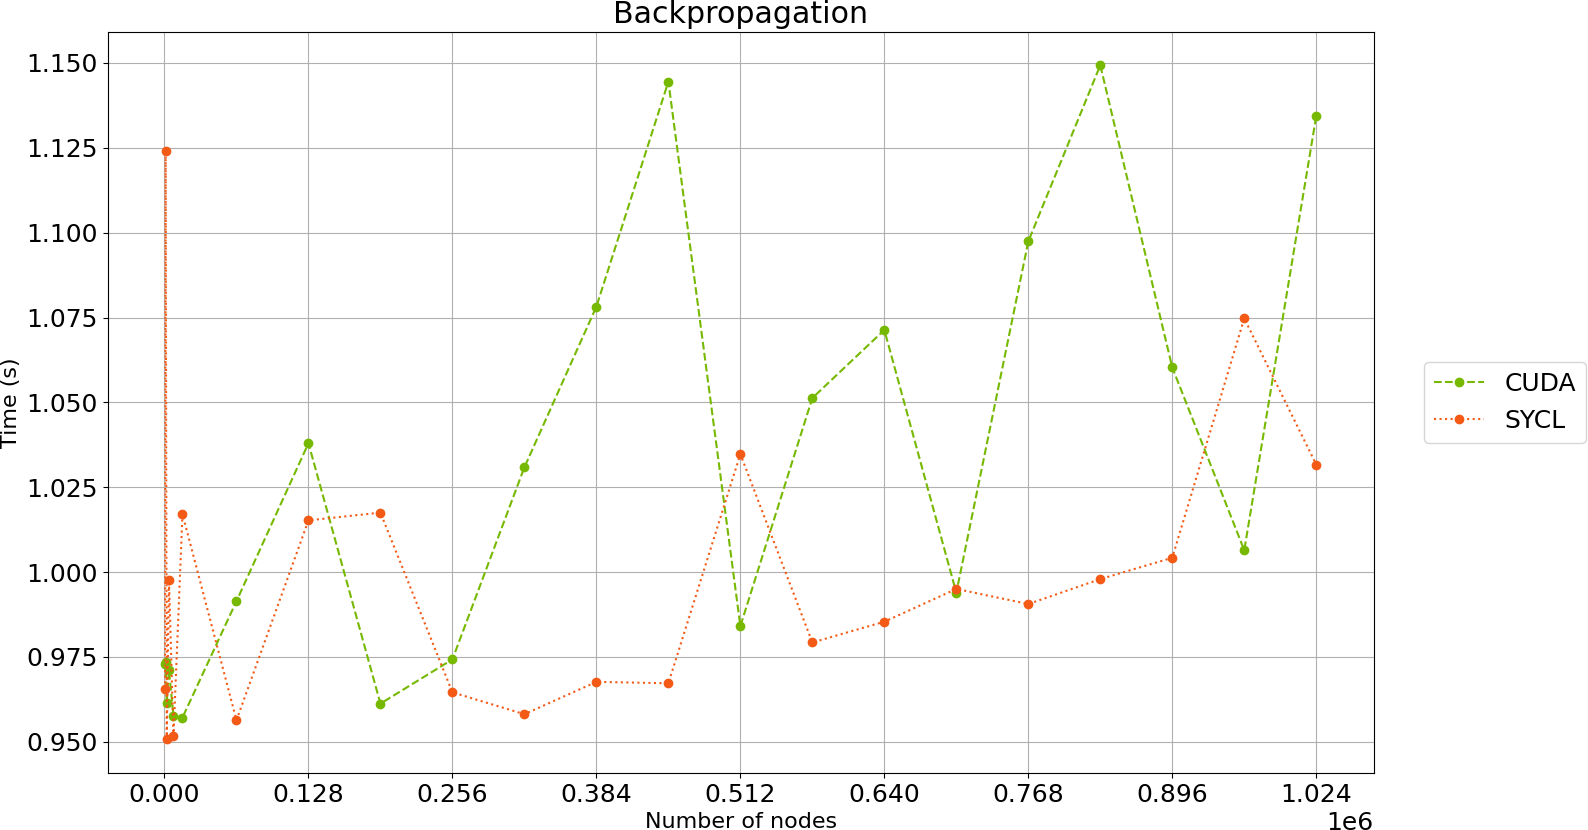
\includegraphics[width=\linewidth]{images/backprop-sycl-cuda.png}
	\caption{Backpropagation benchmark. Results for SYCL and CUDA executions.}
	\label{fig:backprop-sycl-cuda}
\end{figure}

The results in Figure \ref{fig:backprop-sycl-cuda} show a large variation in CUDA/SYCL runtimes for each problem size.
In this experiment, SYCL seems to be a bit more stable in terms of time fluctuation.

The SYCL version of this algorithm has a limitation since the maximum problem size supported is near 1.048.000 nodes, while the CUDA implementation surpasses this constraint.

\lstinputlisting[language=log,style=logstyle,caption={NDRange error on backpropagation benchmark.},label={listing:error-backprop-sycl}]{listings/error_backprop_sycl.log}

This limitation can be evidenced by using \texttt{1,048,800} as the problem size.
Listing \ref{listing:error-backprop-sycl} is the output of this experiment and line 14 shows the root of this limitation.
The problem is that the number of resulting work-groups that the program pretends to create exceeds the maximum established by the compiler.

This constraint is not tied to the SYCL specification but the compiler implementation, which is \texttt{clang++} in this case.
Since the hardware is always a physical and tangible limit, this particular compiler has decided to set an arbitrary limit for this very reason.

One solution to this situation would be to assign more work to each work-group.
This would reduce the number of work-groups so that it does not hit the limit set by the compiler.


